% Chapter 6

\chapter{Multi-lable Classification Methodology} % Write in your own chapter title
\label{Chapter6}
\lhead{Chapter 6. \emph{Methodology}}

\section{Artificial Dataset}

To demonstrate the approach, the dataset, named color detector, is created artificially. To each image, it has three labels for representing colour, $red$, $green$ and $blue$. If an image is red hue, it has a label for $red$ and label values of $green$ and $blue$ are negative. The representation of colour combination follows colour wheels. If an image has a hue close to $purple$, it has positive labels for $red$ and $blue$, and negative label for $green$, and so on.
\graphicspath{ {./Figures/} }
\begin{figure}[!htb]
\centering
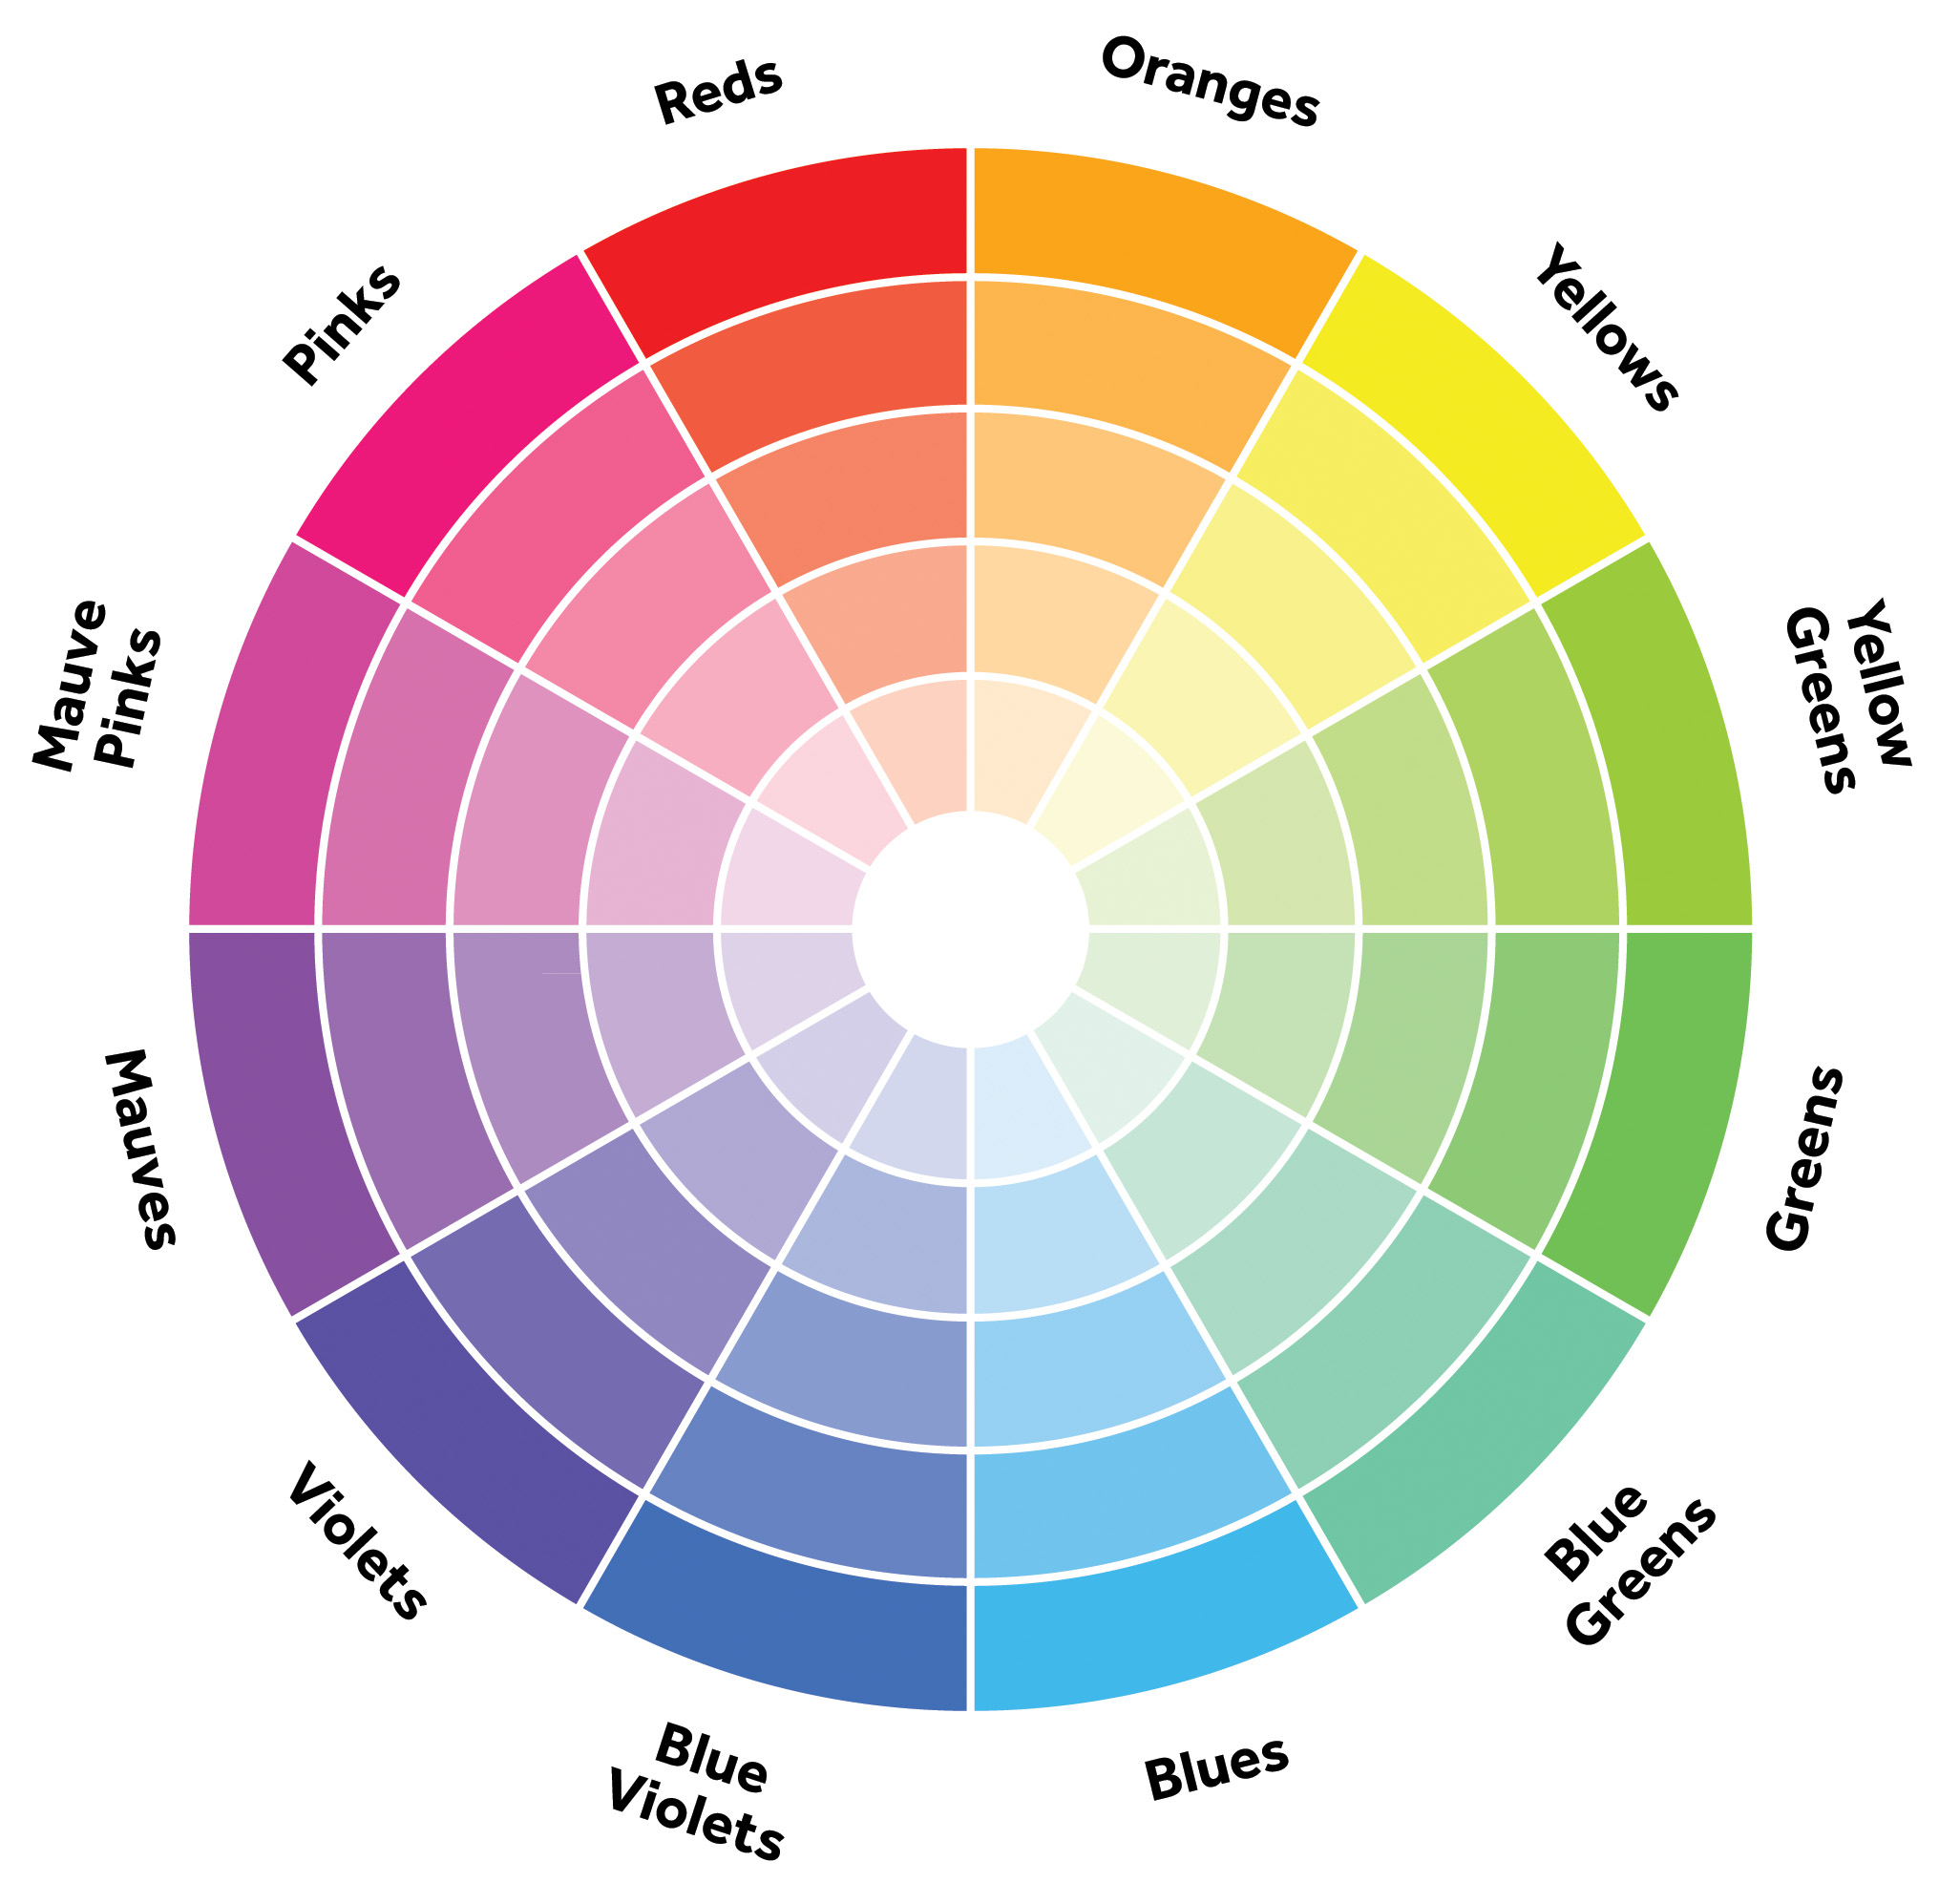
\includegraphics[scale=0.1]{color_wheel.jpg}
\caption{\label{fig:perceptron}Colour Wheel Diagram}
\end{figure}

For each sample $x_{i}$, it owns 3 labels ${y_{0},y_{1},y_{2}} y_{j} \in \{-1,1\}$ which represent $red$, $green$ and $blue$ respectively.

\subsection{Colour Generation}

To generate dataset artificially, we create $16x16$ size images and each image has $256$ pixels. For each pixel, we generate a random floating point number $h$ in the range $[0.0, 1.0)$ and use it as value for Hue via formulation.
\begin{equation}\label{eq:FormulationHue}
H = h + r * 0.4 - 0.2 (r \in [0.0,1.0))
\end{equation}
Where $r$ is another random floating point number. Then we generate 2 random floating point numbers as Saturation(S) and Value(V) values. We transform HSV values to RGB values and time $255$ for each pixel. Repeating the steps, we can get a $256$ pixels image. Because we get a RGB image via converting a HSV image, we compute RGB label value basing on previous $h$.

\graphicspath{ {./Figures/} }
\begin{figure}[!htb]
\centering     %%% not \center
\subfigure[L:-1 -1 1]{\label{fig:a}
\includegraphics[width=0.3\textwidth]{0}}
\subfigure[L:-1 1 1]{\label{fig:b}
\includegraphics[width=0.3\textwidth]{1}}
\subfigure[L:-1 1 -1]{\label{fig:c}
\includegraphics[width=0.3\textwidth]{3}}
\caption{Multi-label Samples. Left image is a blue one, middle one is green plus blue and right one is green.}
\end{figure}

The dataset contains $1000$ images in total. $960$ images are training samples and $40$ are test samples. 




















